\section{The whole macromolecule}
\label{wholemacromolecule}

To regenerate the whole human \ttt{metHgb} macromolecule, we are going to follow basically the schema shown in \ffigure{fig:scipion_workflow_whole_reconstruction}. Starting from the symmetric unit, \chimera \ttt{operate} protocol allows to generate the whole molecule by symmetry. As in the previous step, validation programs drive to selection of the best $model$ of the whole molecule after one or several rounds of assessment - refinement -assessment. A final validation step will be accomplished with \chimera \ttt{map subtraction} protocol to assess the volume density occupancy of the new macromolecule generated.

\begin{itemize}

 \item Protocol \scommand{chimerax - operate} to generate the whole molecule of human \ttt{Hgb}:\\
 
 Following previous instructions, open \chimera \ttt{operate} protocol (\ffigure{fig:chimera_operate_protocol} (1)), load 
 the selected atomic structure $model$ of \ttt{metHgb} asymmetric unit (2), and execute the protocol (3). \chimera graphics interface will show you the $model$ of \ttt{metHgb} asymmetric unit. Considering the C2 symmetry of the whole molecule, write in \chimera command line to re-generate the whole molecule:\\
 
 \ttt{sym \#2 C2 copies true}\\
 
 A symmetric image of the input $model$ (\ffigure{fig:chimera_operate_sym}; $model$ \ttt{\#2}) will be generated. The new $model$ \ttt{\#3} contains both the input (\ffigure{fig:chimera_operate_sym}, \iii{model} \ttt{\#3.1})and the symmetric unit (\iii{model} \ttt{\#3.2}). 
 
 \begin{figure}[H]
    \centering 
    \captionsetup{width=.9\linewidth} 
    \includegraphics[width=0.50\textwidth]{Images/Fig41}
    \caption{$Model$ generated for the whole human \ttt{metHgb}.}
    \label{fig:chimera_operate_sym}
   \end{figure}
Although the whole structure can be saved by writing in \chimera command line \ttt{scipionwrite \#3 prefix whole\_model\_} to have only one \iii{model} and not a group of two \iii{models}, we will write in in \chimera command line:\\
 
 \ttt{rename \#3.1 id \#4}\\
 \ttt{rename \#3.2 id \#5}\\
 \ttt{scipioncombine \#4,5}\\
 \ttt{scipionwrite \#6 prefix whole\_model\_}\\
 
 \ttt{Note}: In this small example selected for modeling it doesn't matter if we model the map asymmetric unit or the whole molecule. However, in real life to model the whole molecule doesn't make sense because of its huge size. In that case, we will limit our modeling to the map asymmetric unit. The right modeling of this part of the molecule will require to add the adjacent asymmetric units in order to perform the appropriate modeling of the overlapping areas, avoiding steric classes in the reconstruction by symmetry of the whole molecule. In that case, the command lines would be:
    \begin{itemize}
     \item To generate the symmetry copies:\\
     \ttt{sym \#2 C2 copies true}\\
      \item To remove in the new \iii{model} \ttt{\#3} the symmetry copies with centers within a certain range of distance \ttt{d} of the center of the molecule input \iii{model}:\\
      \ttt{delete \#3 \& \#2 \#>d}
    \end{itemize}
At this point we will continue with the refinement process of this asymmetric unit plus neighbors. The validation will focus only in the asymmetric unit, which will be recovered by removing the remaining adjacent asymmetric units. This cleaning or removing of the neighbor units can be performed with the protocol \chimera \ttt{operate} each time we would like to validate the structure.
 
 
 \item Protocols to refine the new combined structure generated:\\
  
As we said in the previous chapter regarding the building of the asymmetric unit, refinements should cover specially the overlapping areas, in this case between the two asymmetric units. Help yourself with the \coot tools of \ttt{Validate} in the main menu, as well as the visualization tools of \phenix \ttt{real space refine} protocol.\\

\ttt{Note}: Look at the name of chains before saving the atomic structure in \coot. If the symmetric copies of chains \ttt{A} and \ttt{B} are called \ttt{A002} and \ttt{B002}, respectively, changing these names to \ttt{C} and \ttt{D} is recommended.
 \item Validation protocols to select the best $model$ of the whole human \ttt{Hgb}:\\
 
 \emringer and $Validation CryoEM (MolProbity)$ statistics have to be computed for the new $model$ of the whole human \ttt{metHgb} obtained by using \chimera \ttt{operate} protocol (see results \ttable{table:refmac_question_12} in Appendix \ref{app:solutions}; \textbf{Question \ref{wholemacromolecule}\_1}). Because of high values of \ccmask and \emringer \ttt{score}, as well as acceptable \molprobity statistics, $model$ generated by \chimera \ttt{operate} protocol is selected as $model$ of the whole human \ttt{metHgb}. Additional refinement steps with \phenix \ttt{real space refine} and \refmac do not seem to improve the result significantly. In this case, the RMSD value of the selected atomic structure $model$, regarding the published structure, yields an intermediate value between the best and the worst one.\\
 
 \item Protocol \scommand{chimerax - map subtraction} to assess volume density occupancy:\\
 
 We perform this analysis in order to identify parts of the density map that were not modeled previously, maybe unknown parts of the complex, although areas where the \iii{model} doesn't fit the map can be also identified. Sometimes the density level or the resolution in these areas differ from the rest of the map and commonly are more blurry, which makes them much more difficult to identify and trace. Ideally, we would like to remove the map density associated to the already traced atomic structure to facilitate the modeling of the remnant density. Obviously, there are some limitations in this process because the structure-derived map might not be absolutely identical to the reconstructed map. As one possible aproximation, we will run a protocol based on \chimera (see Appendix \ref{app:chimeraMapSubtraction} with use cases) to subtract the modeled part of the map from the whole map.
 
 First, open the \chimera \ttt{map subtraction} protocol (\ffigure{fig:chimera_map_subtract} (1)), load both the initial map obtained from the reconstruction process (2) and its resolution. Although in this case we are going to consider the nominal map resolution, in real life you should test different resolution values among which the half value of the resolution obtained by FSC is recommended. Include also the refined atomic structure $model$ of the whole human \ttt{metHgb} (3). As a control of the subtraction process we are going to remove 7 residues of the chain \ttt{A}. With this aim, use the three wizards on the right (4) to select that chain and residues located between positions \ttt{22} and \ttt{28}, both included. Since we are interested in observing differences in the whole map, the default option \ttt{No} will be maintained regarding the selection of a map fraction around the atomic structure (5). Then, execute the protocol (6). 
 
 \begin{figure}[H]
    \centering 
    \captionsetup{width=.9\linewidth} 
    \includegraphics[width=1\textwidth]{Images/Fig42}
    \caption{Completing the protocol \scommand{chimerax - map subtraction}.}
    \label{fig:chimera_map_subtract}
   \end{figure}
   
\chimera graphics window will open and the commands driving the subtraction process will be applied. The \ffigure{fig:chimera_map_subtract_2} shows in blue the map resulting from subtracting the \iii{model}-derived map from the starting map \ttt{EMD-3488} after applying a Gaussian filter. Three main map bodies can be observed moving the density threshold of this map (model \ttt{\#9} in the \ttt{Models} panel). The red arrow number \ttt{1} points to the control map derived from removing 7 residues of the chain \ttt{A} of the atomic structure. The other two red arrows (number \ttt{2}) point to two unexpected remnant densities. 

  \begin{figure}[H]
    \centering 
    \captionsetup{width=.9\linewidth} 
    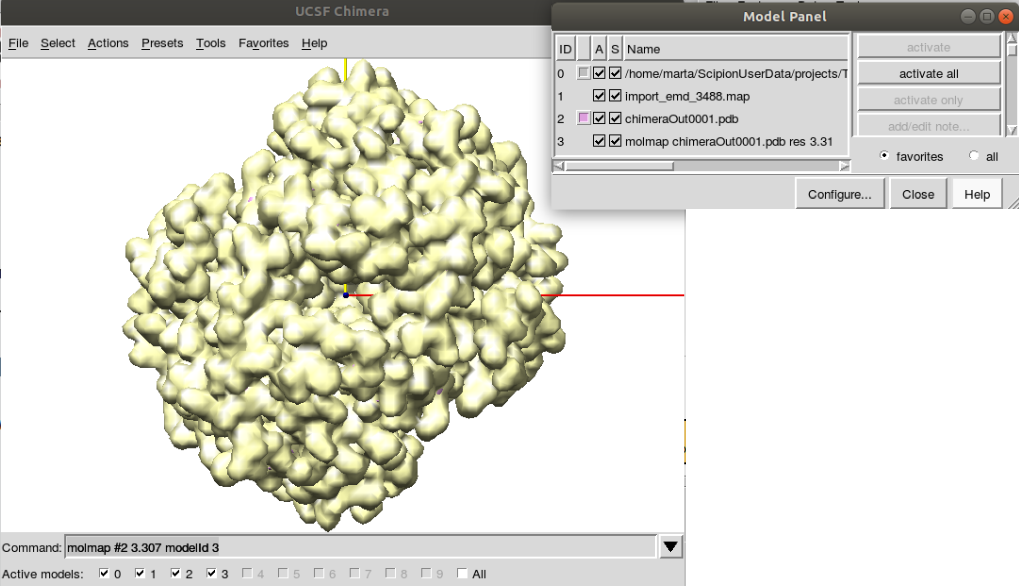
\includegraphics[width=0.90\textwidth]{Images/Fig43}
    \caption{Filtered subtraction map (blue bodies) and refined atomic structure (pink) of the whole human \ttt{Hgb}.}
    \label{fig:chimera_map_subtract_2}
   \end{figure}

The two additional bodies of density should not appear with an appropriate modeling of the human \ttt{Hgb} showing acceptable validation scores. However, in this final \iii{model} of the whole human \ttt{Hgb} we didn't refine on purpose the C-terminal ends of chain \ttt{A} and its symmetric chain \ttt{C}. The \ttt{ARG} residues don't fit to the map density and the remnant densities identified in the subtraction protocol correspond to the C-terminal ends of chains \ttt{A} and \ttt{C}. A fair tracing of those parts of the molecule would avoid remnant densities others than the control. To check the right tracing of the human \ttt{Hgb} we have overlapped the above mentioned published atomic structure of the human \ttt{Hgb} (\ttt{PDB ID 5NI1}), in green in the \ffigure{fig:chimera_map_subtract_3}, and our final \iii{model}, depicted in pink. The zoom in details the C-terminal end of our \iii{model} (red arrow) and the published one (green arrow), which perfectly fits the body of density. 

  
  \begin{figure}[H]
    \centering 
    \captionsetup{width=.9\linewidth} 
    \includegraphics[width=0.90\textwidth]{Images/Fig44}
    \caption{Overlapping structures of the models built (pink) and published (green) of the whole human \ttt{Hgb}. Zoom in to detail the C-terminal end of the chain \ttt{C}.}
    \label{fig:chimera_map_subtract_3}
   \end{figure}

   As a conclusion, if you do not have additional densities with the example of this tutorial, except the control one, you'd have performed a good modeling and you could use your atomic structure to perform other types of analyses and to publish it. Otherwise, you should still refine your \iii{model}.
 
\end{itemize}
